\section*{1. Introduction}
\subsection*{Patter Recognition Pipeline}
\begin{figure}[H]
    \centering
    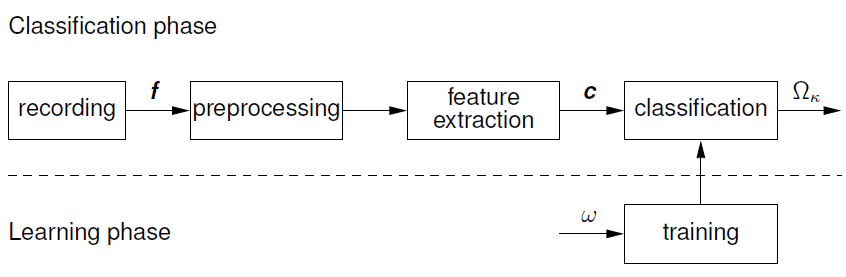
\includegraphics[scale=0.6]{figures/pipeline}
\end{figure}

\subsection*{Posulates of Pattern Recognition}
\begin{enumerate}
    \item
        Availability of a representative sample $\omega$ of patterns $^if(x)$ for a given field of problems $\Omega$
        $$\omega = \{^1f(x),\dots,^Nf(x)\}\subseteq \Omega$$
    \item
        A (simple) pattern has features, which characterize its membership in a certain class $\Omega_{\kappa}$
    \item
        Compact domain in the feature space of features of the same class;\\ 
        domains of different classes are (reasonably) seperable.
        \begin{itemize}
            \item
                small intra-class distance
            \item
                high inter-class distance
        \end{itemize}
    \item
        A (complex) pattern consists of simpler consituents, which have certain relations to each other. A pattern may be decomposed into the constituents.
    \item
        A (complex) pattern $f(x) \in \Omega$ has a certain structure. Not any arrangement of simple constituents is a valid pattern. Many patterns may be represented with relatively few constituents.
    \item
        Two patterns are similar if their features or simpler constituents differ only lightly.
\end{enumerate}

\subsection*{Performance Evaluation}
\begin{itemize}
%    \item
%        General confusion matrix:
%\begin{figure}[H]
%    \centering
%    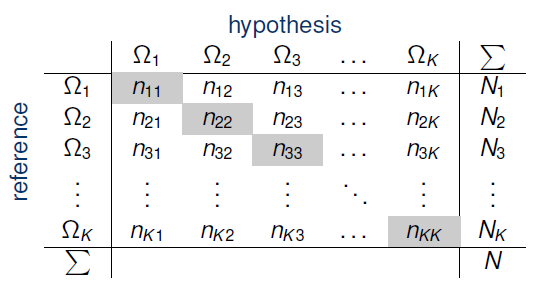
\includegraphics[scale=0.7]{figures/conf_general}
%\end{figure}
    \item
        Two class confusion matrix:
\begin{figure}[H]
    \centering
    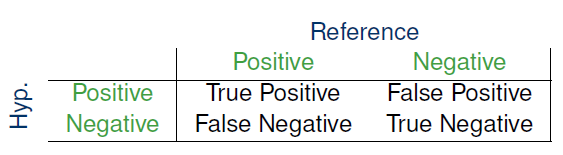
\includegraphics[scale=0.7]{figures/conf_two}
\end{figure}
    \item
        Performance measures:
        \begin{itemize}
            \item
                TP rate (recall, sensitivity):  $\ffrac{\#TP}{\#TP + \#FN}$
            \item
                FP rate (false alarm rate):  $\ffrac{\#FP}{\#FP+\#TN}$ 
            \item
                TN rate (specifity): $\ffrac{\#TN}{\#FP+\#TN}$ = 1 - false positive rate
            \item
                Precision: $\ffrac{\#TP}{\#TP+\#FP}$ 
            \item
                Negative prediction value: $\ffrac{\#TN}{\#TN+\#FN}$
            \item
                Accuracy: $$ACC = \ffrac{\#TP + \#TN}{\#TP + \#FP + \#FN + \#TN}$$ 
            \item
                F-measure: harmonic mean of recall and precision: $$F = \ffrac{2\cdot \text{recall} \cdot \text{precision}}{\text{recall} + \text{precision}}$$
        \end{itemize}
    \item
        Receiver Operation Characteristics (ROC) Curves: A classifier defined a single 2-d point (y-axis: TP rate)
        \begin{figure}[H]
            \centering
            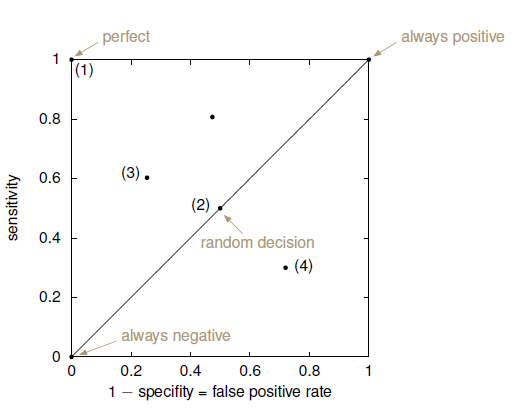
\includegraphics[scale=0.7]{figures/roc1}
        \end{figure}
    \item
        Compute ROC curve of classifier: Varying threshold results in varying TPR/FPR
        \begin{figure}[H]
            \centering
            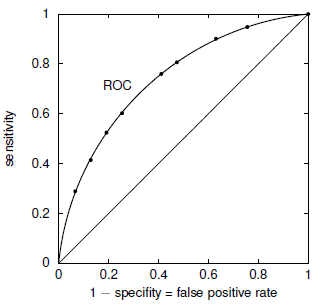
\includegraphics[scale=0.7]{figures/roc2}
        \end{figure}
    \item
        Performance measure: area under curve (AUC)

\end{itemize}

